\section{NP-Hardness}

\subsection{A Game You Can't Win}
Given a box with $n$ binary switches and a light bulb.
Inside the box is a boolean circuit, s.t
\begin{itemize}
    \item \textsc{And}, \textsc{Or}, \textsc{Not} gates, as shown in \cref{fig:gates};
    \item $n$ input wires, one per switch;
    \item Gates connected to single output, i.e the light bulb.
\end{itemize}
\begin{figure}[H]
    \centering
    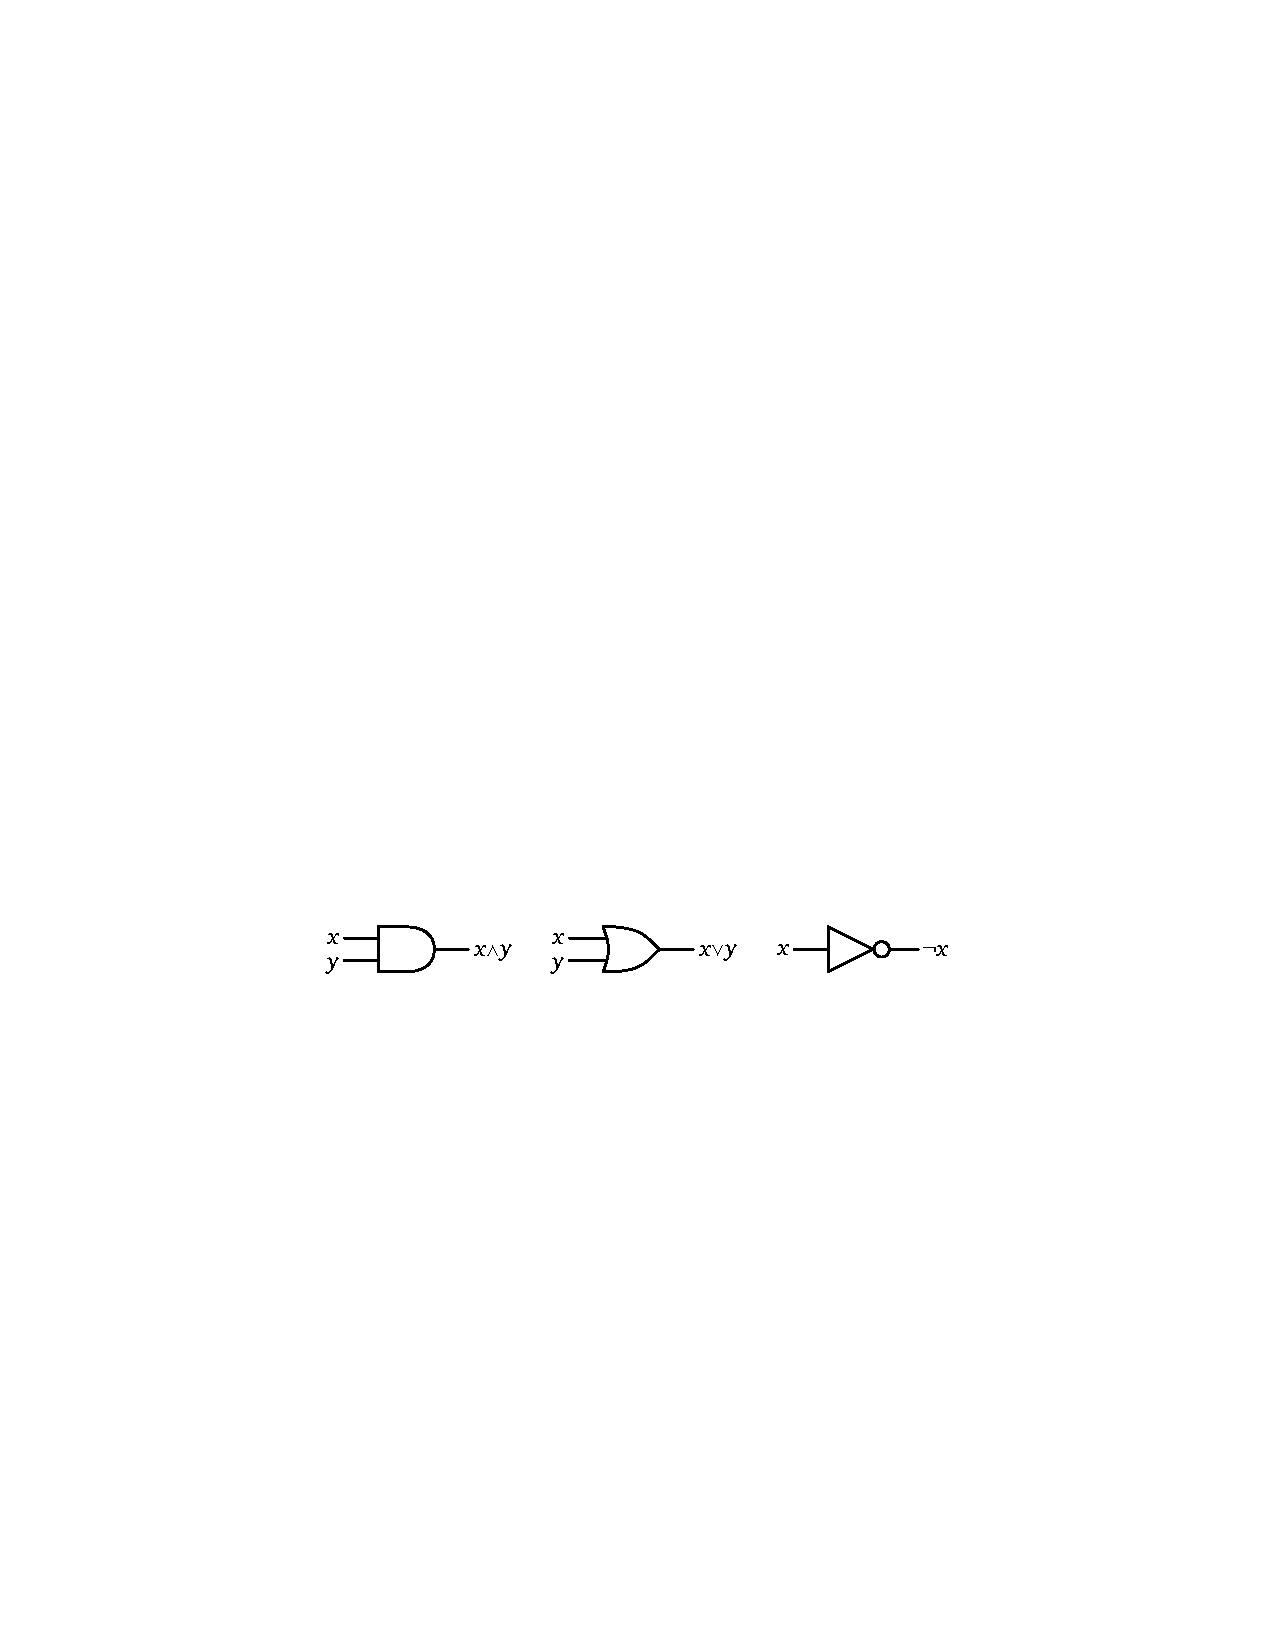
\includegraphics{fig/gates}
    \caption{An \textsc{And}, an \textsc{Or}, and a \textsc{Not} gate}
    \label{fig:gates}
\end{figure}
An example is shown in \cref{fig:lightbulb}
\begin{figure}[H]
    \centering
    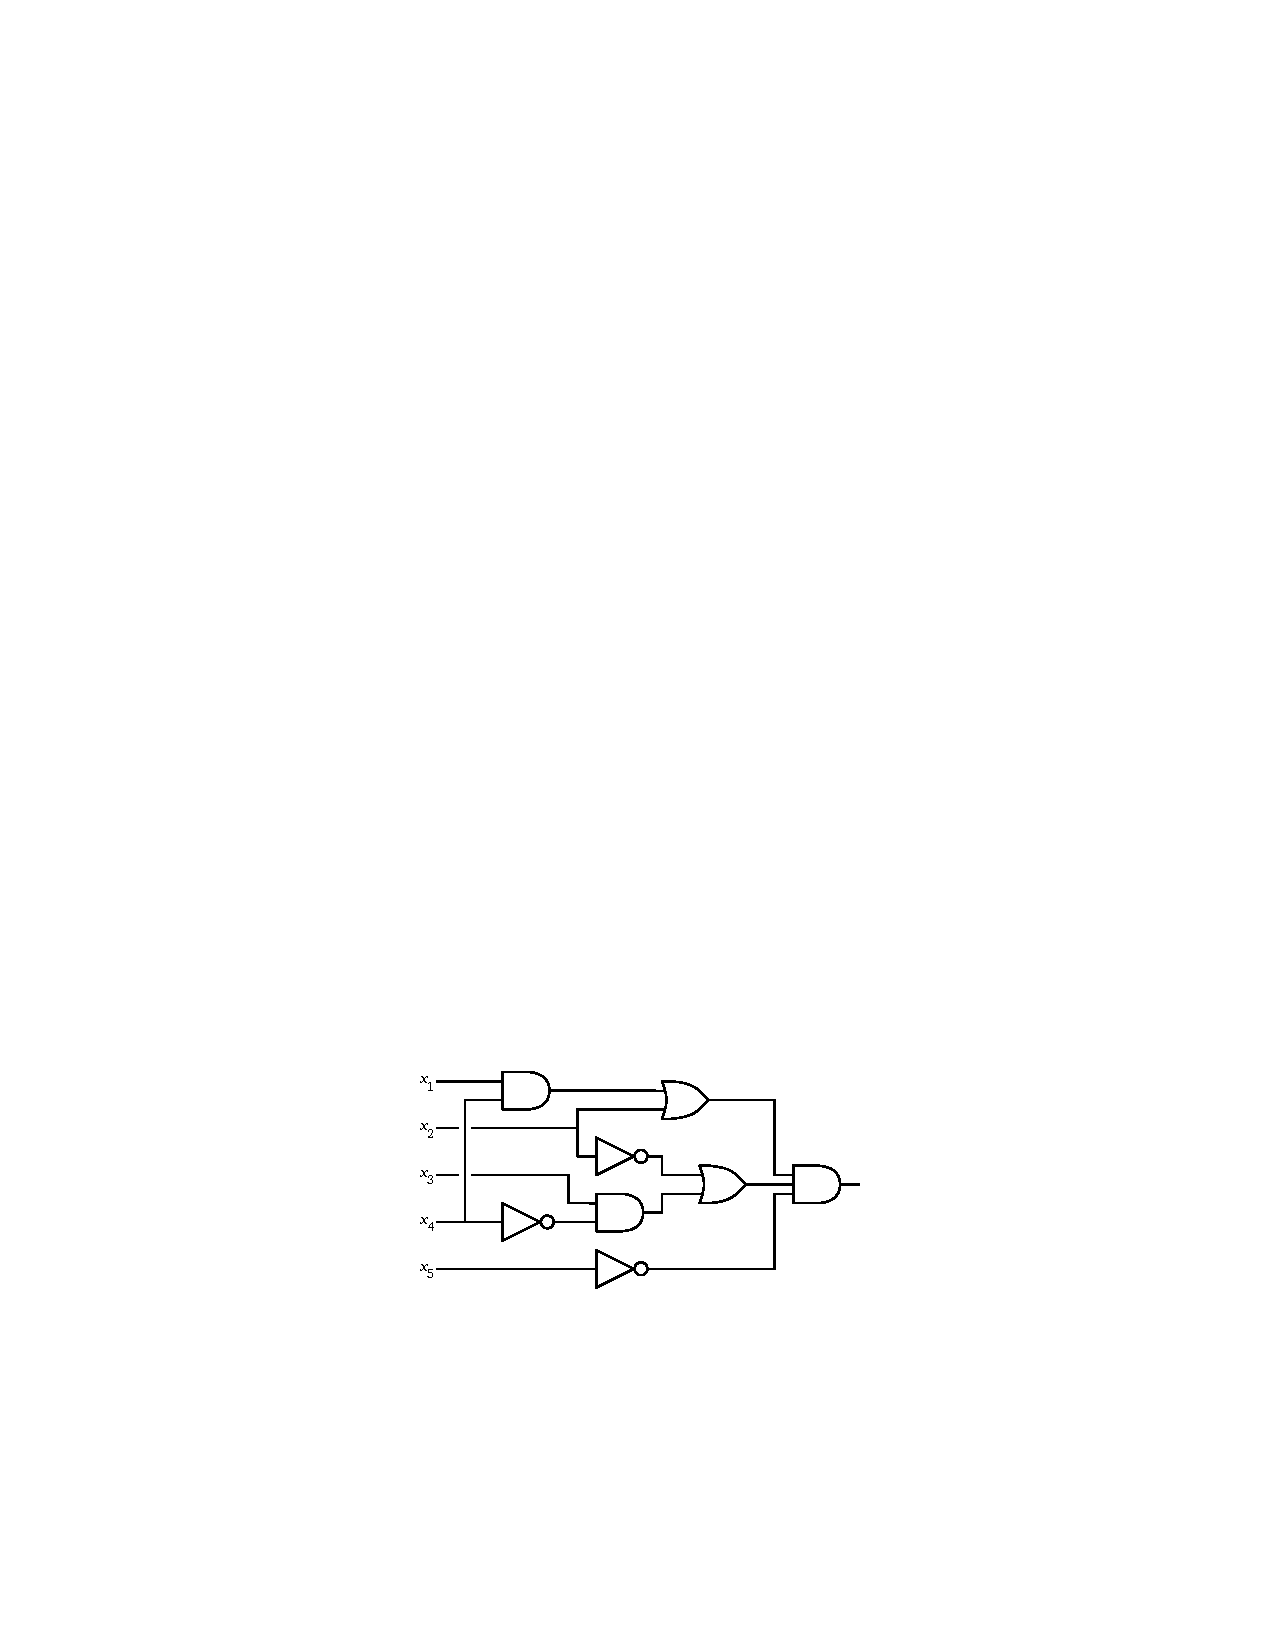
\includegraphics[scale=1.5]{fig/lightbulb}
    \caption{A boolean circuit}
    \label{fig:lightbulb}
\end{figure}
We want to know if there is a way to set switches s.t
light bulb turns on.
There are $2^n$ possible binary inputs. There is an \bigO{n} size circuit
which accepts a single strings and rejects all others.
Hence, if you cannot see inside, in worst case you must try all $2^n$ strings.

Suppose now you can see inside box. Can you do better than guessing all strings?
The answer is nobody knows for sure but many believe not.

The problem of determining if boolean circuit has satisfying assignment is all
\textsc{CircuitSAT}.

\subsection{P versus NP}
Minimum for an algorithm to be efficient is that it runs in polynomial time,
i.e \bigO{n^c} for constant $c$, $n$ is input size.
In this course, we focused on problems with polynomial solutions where $c$ is small.
\begin{itemize}
    \item Some problems known to require exponential time, i.e \bigO{c^n}, $c>1$.
    \item Some problems cannot even be solved (for example, Halting Problem).
    \item Some problems we don't know how hard.
\end{itemize}
NP-hard is a class most believe cannot be solved in polynomial time,
but no one knows for sure.

A decision problem is a problem whose output is a single boolean value,
i.e. \textsc{Yes/No}.
For example: LIS was an optimization problem. $\rightarrow$ ``Is there any increasing sequence of length $\geq k$?''
is a decision problem.
\begin{itemize}[leftmargin=.75in]
    \item[P] Set of decision solvable in polynomial time, i.e ``efficiently solvable''.
    \item[NP] Decision problems s.t if answer in \textsc{Yes}, then there is a proof
        that can be checked in polynomial time. $\rightarrow$ can verify \textsc{Yes} if proof given to us.
    \item[Co-NP] Decision problems s.t if answer in \textsc{No}, then there is a proof
        that can be checked in polynomial time. $\rightarrow$ can verify \textsc{No} if proof given to us.
\end{itemize}
\textsc{CircuitSAT} is in NP, if satisfying string, then given string, it is easy to verify.

Why do most believe $P \neq NP$?
One intuition is that: solving problems is harder than verifying solutions.
\begin{itemize}[leftmargin=.75in]
    \item[P] Problem in CLRS that you can solve quickly.
    \item[NP] Problem in CLRS that you can verify solution quickly.
\end{itemize}

\subsection{NP-Hard/NP-Complete}
A problem $\Pi$ is NP-hard if a polynomial time algorithm for $\Pi$ implies
polynomial time algorithm for all problems in NP.
\begin{quote}
    $\Pi$ is NP-hard $\leftrightarrow$ If $\Pi$ solution in polynomial time, then P = NP.
\end{quote}

Hence, most believe no NP-hard problem solvable in polynomial time.

$\Pi$ is NP-complete if $\Pi$ is NP-hard and $\Pi \in \text{NP}$.

Thousands of problems have been shown to be NPC.
How does one prove something NP-hard or NPC?

\begin{theorem}[Cook-Levin Theorem] \textsc{CircuitSAT} is NPC.\end{theorem}

All problems that are shown to be NPC, reduce from \textsc{CircuitSAT}.

\subsection{Reductions \& SAT}
To prove any problem other than the \textsc{CircuitSAT} is NP-hard, use reduction.
Reducing problem A to problem B means solving A using solution for B.
To prove B is NP-hard, reduce \underline{from} known NP-hard problem A \underline{to} problem B.
Require reduction to be polynomial time in the A instance size.

Intuition: we are sure A is hard, Hence B must be hard, since otherwise it implies A can be
solved quickly.

Often write: $B \geq_p A$,
$\geq_p$ stands for B at least as hard as A ignoring polynomial factor.

A may still require more time to solve bu not more than polynomial factor.

Given a boolean formula, is there a satisfying assignment,
i.e a binary assignment variables evaluating to be true.
For example: 
\[(a \lor b \lor c \lor \overline{d}) \Longleftrightarrow ((b \land \overline{c}) \lor \overline{(\overline{a} \Rightarrow d)} \lor (c \neq a \land b))\]
To prove SAT is NP-hard, we reduce from \textsc{CircuitSAT}.
So given a boolean circuit (i.e. a DAG), we must convert to an equivalent boolean formula.

One solution: circuit has single output gate,
so start at root gate, recursively write formula,
for each subtree and combine formula with root gate operation.
This method takes exponential time since DAG, not a tree.

Here is the polynomial time reduction:
\begin{enumerate}
    \item For each gate output wire create a variable: $y_1 \ldots y_n$ as gates outputs,
        $x_1 \ldots x_m$ as circuit input, $z$ as circuit output.
    \item For each gate wire clause saying inputs match output.
    \item Take \textsc{And} of all these clauses and $z$.
    \item This says all gates work properly and output is $1$.
\end{enumerate}
For example, \cref{fig:sat} shows the formula transformed from \cref{fig:lightbulb}.
\begin{figure}[H]
    \centering
    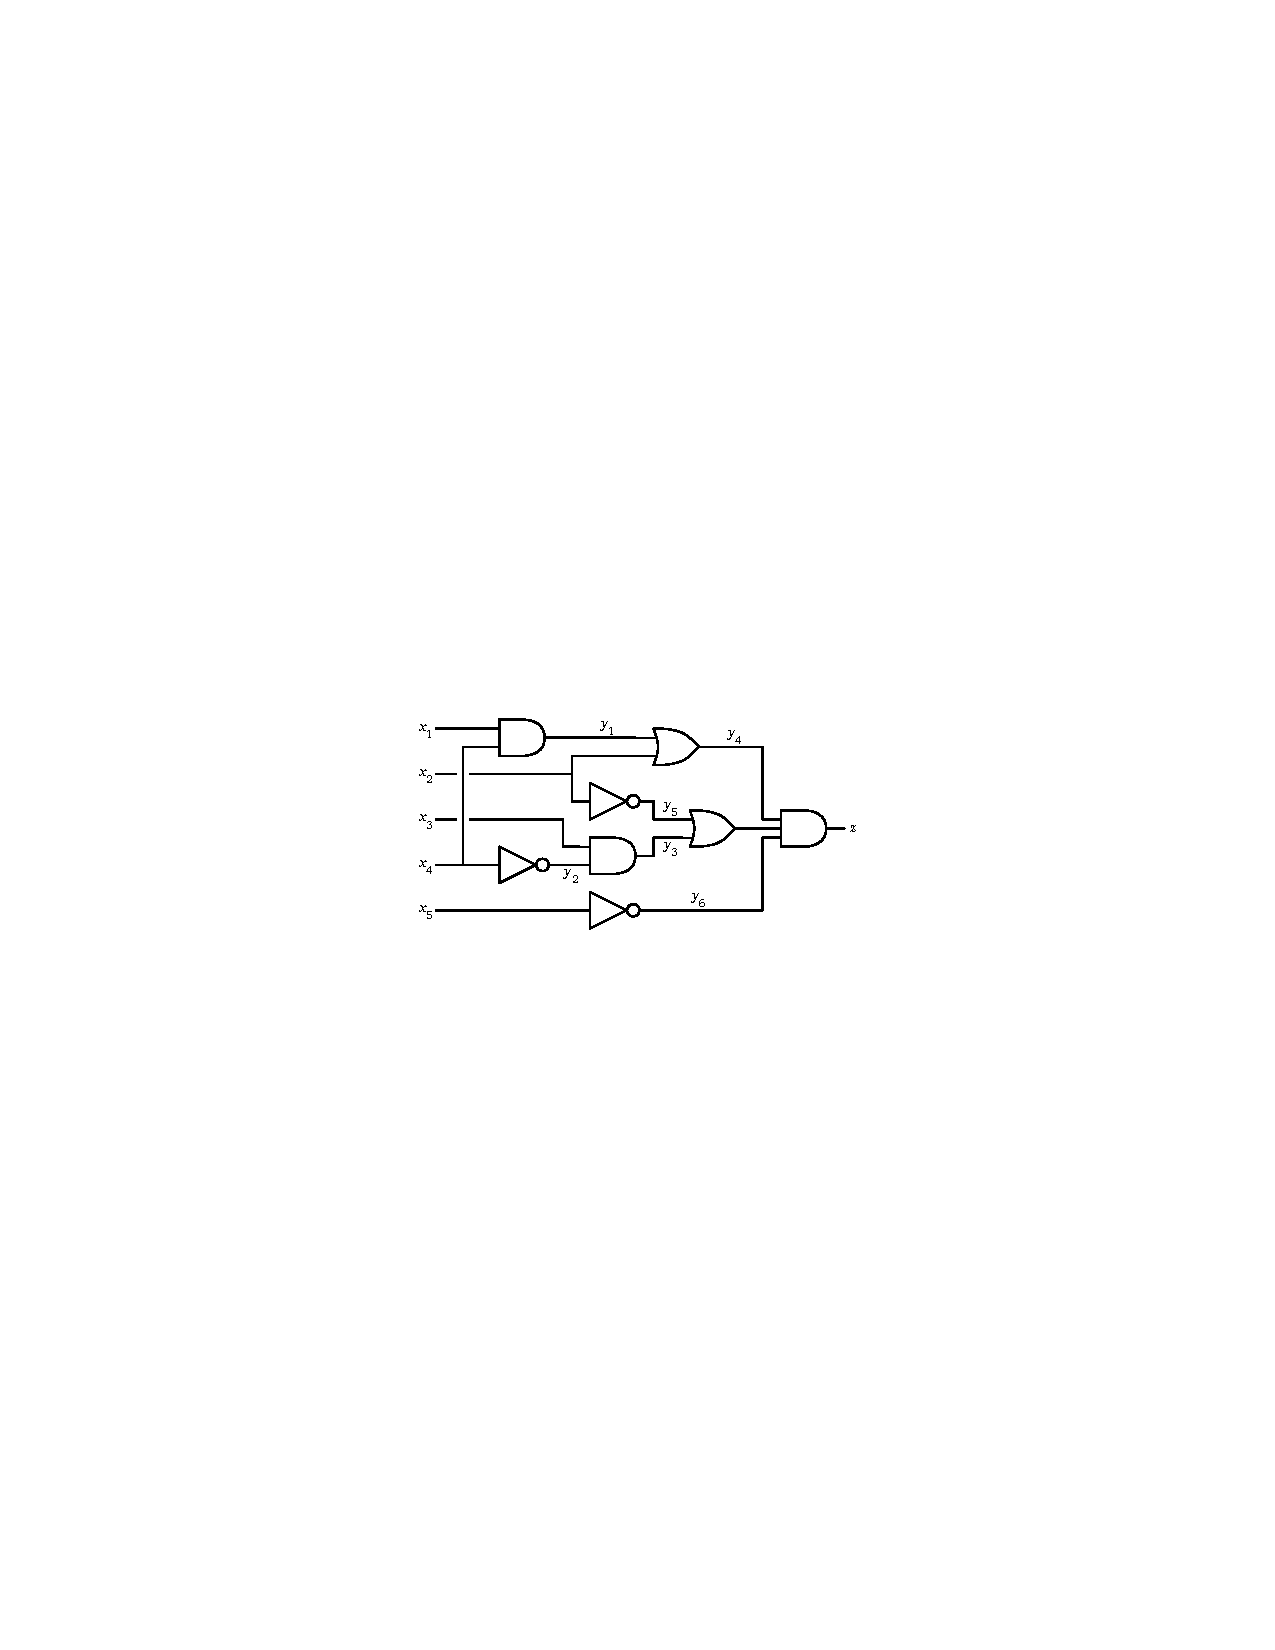
\includegraphics[scale=1.25]{fig/sat}
\begin{align*}
    (y_1 = x_1 \land x_4)\land&(y_2 = \overline{x_4})\land(y_3 = x_3 \land y_2)\land(y_4 = y_1 \land x_2)\land\\
    &(y_5 = \overline{x_2})\land(y_6 = \overline{x_5})\land(y_7 = y3 \lor y_5)\land(z = y_4 \land y_7 \land y_6) \land z
\end{align*}
    \caption{A boolean circuit with gate variables added, and an equivalent boolean formula}
    \label{fig:sat}
\end{figure}
The original circuit is satisfiable if and only if the boolean formula is.
\begin{itemize}[leftmargin=.75in]
    \item[$\Longrightarrow$] Given satisfying assignment to circuit, can find satisfying assignment to formula
        by computing output of every gate.
    \item[$\Longleftarrow$] Given satisfying assignment to formula, just ignore $y_i$s and $z$ to get circuit input.
\end{itemize}
By this, we can produce formula from circuit in linear time.
Thus, polynomial time reduction from \textsc{CircuitSAT} to SAT.

\subsection{3SAT}
Boolean formula is in conjunctive normal form (CNF) if it is the
conjunction (\textsc{And}) of clause,
each of which is a disjunction (\textsc{Or}) of literals,
each of which is a variable of its negation.

A 3CNF formula is a CNF formula with exactly 3 literals per clause.

\begin{theorem}
    3SAT is NP-complete.
\end{theorem}
\begin{proof}
To prove 3SAT $\in$ NP, given satisfying assignment, plug in values and evaluate.

To prove 3SAT is NP-hard: (reduce from \textsc{CircuitSAT})

Given \textsc{CircuitSAT} instance, convert to 3SAT instance:
Assume each gate has fan in at most 2.
\begin{enumerate}
    \item Write circuit as formula with one clause per gate;
    \item Change each gate clause to CNF:
        \begin{align*}
            a=b \land c &\Longleftrightarrow (a \lor \overline{b} \lor \overline{c}) \land
                (\overline{a} \lor b) \land (\overline{a} \lor c) \\
            a=b \lor c &\Longleftrightarrow (\overline{a} \lor b \lor c) \land
                (a \lor \overline{b}) \land (a \lor \overline{c}) \\
            a = \overline{b} &\Longleftrightarrow (a \lor b) \land (\overline{a} \lor \overline{b})
        \end{align*}
    \item Convert to 3CNF (exactly 3 literals per clause)
        \begin{align*}
            a &\Longleftrightarrow (a \lor x \lor y) \land (a \lor \overline{x} \lor y) \land
                (a \lor x \lor \overline{y}) \land (a \lor \overline{x} \lor \overline{y}) \\
            a \lor b &\Longleftrightarrow (a \lor b \lor x) \land (a \lor b \lor \overline{x})
        \end{align*}
\end{enumerate}
Polynomial time reduction, hence 3SAT is NP-hard.
\end{proof}

\subsection{Independent Set}
Let $G$ be an undirected graph. An independent set in $G$ is a set of vertices
with no edge between them.

\noindent\textbf{Independent Set Problem}: Given $G$ and integer $k$, is there an independent set of size $\geq k$.

\noindent\textbf{Max Independent Set Problem}: Given $G$, find the size of largest independent set.

\begin{proof}
We prove the Independent Set Problem is NP-hard by reducing from 3SAT:
Input is a 3SAT instance with $x$ clauses.
For each literal of each clause, create a vertex.
Add an edge between two vertices if either:
\begin{itemize}
    \item literals are in the same clause;
    \item literal correspond to variable and its negation.
\end{itemize}
For example the following formula
\[(a \lor b \lor c) \land (b \lor \overline{c} \lor \overline{d}) \land
    (\overline{a} \lor c \lor d) \land (a \lor \overline{b} \lor \overline{d})\]
is transformed into the following graph:

\begin{figure}[H]
    \centering
    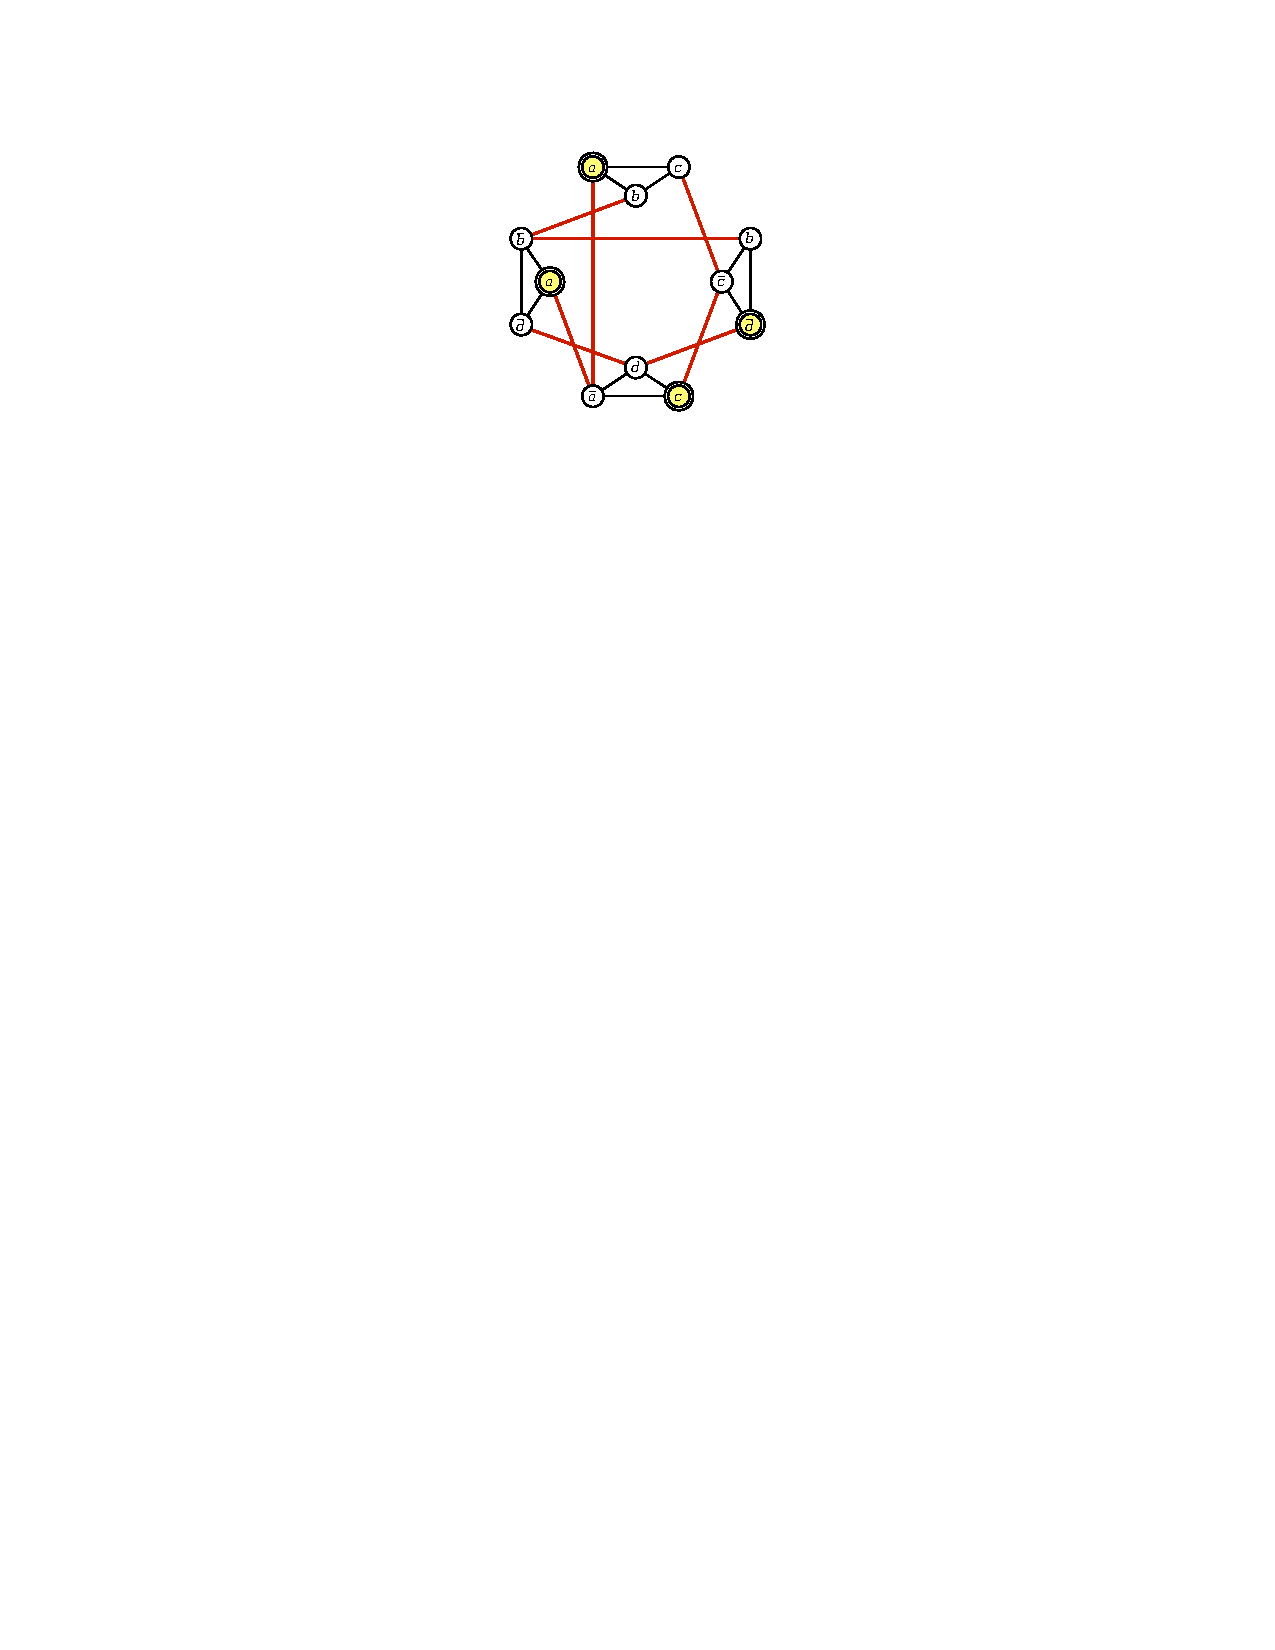
\includegraphics[scale=1.5]{fig/indepset}
    \caption{A graph derived from a 3CNF, and an independent set of size 4}
    \label{fig:indepset}
\end{figure}

The formula is satisfiable if and only if independent set of size $x$:
\begin{itemize}[leftmargin=.75in]
    \item[$\Longrightarrow$] To get satisfying assignment, set each literal from
        independent set to be true.\\
        Since contradictory literals connected by edge, this assignment consistent.\\
        The formula is evaluated to be true since each clause satisfied.
    \item[$\Longleftarrow$] If there is a satisfying assignment, choose one literal for
        each clause that is true.\\
        These literal are independent set in graph since from different clauses and consistent.
\end{itemize}

This proves \textsc{IndepSet}(G,K) is NP-hard.

Since given a subset, can easily check if it is independent set and size $\geq k$,
\textsc{IndepSet}(G,K) $\in$ NP.

Hence, \textsc{IndepSet} in NP-complete.
\end{proof}

\subsection{Clique}
A clique is a subset of vertices where every pair connected.
MaxClique asks for size of largest clique.

\textsc{Clique} is NPC.

Define complement graph $\overline{G}$ as a vertex set, where edge is in $\overline{G}$ if and only if
the edge is not in $G$.
A set if vertices is independent set of $G$ if and only if the same set of vertices is clique in $\overline{G}$.

\subsection{Vertex Cover}
A vertex cover is a set of vertices such that every edge in $G$ is adjacent to vertex in set.
Minimum vertex cover asks for size of smallest vertex cover.
\textsc{VertexCover} asks if vertex cover of size $\leq k$.

\begin{claim}
    A set $I \subseteq V$ is independent set if and only if $V \setminus I$ is the vertex cover.
\end{claim}

\begin{itemize}[leftmargin=.75in]
    \item[$\Longrightarrow$] Consider edge $uv$, cannot have both $u$ and $v \in I$,
        so at least one endpoint in $V \setminus I$.
    \item[$\Longleftarrow$] If $i$ is not independent set, then for some edge $uv$,
        $u,v \in I$, hence $uv$ not covered in $V \setminus I$, (not vertex cover).
\end{itemize}

Hence, \textsc{IndepSet} of size $\geq k$ if and only if vertex cover of size $\leq n-k$.
$I_{max}$ independent set if and only $V \setminus I$ is minimum vertex cover.

\subsection{Some Intuition}
The reduction tree of the problems discussed in the note and homework is shown in \cref{fig:redtree}.

\begin{figure}[H]
    \caption{Reduction Tree}\label{fig:redtree}
    \centering
    \begin{tikzpicture}[every tree node/.style={draw=none},level distance = 1.5cm]
        \Tree [.\textsc{CircuitSAT}
            [.SAT ]
            [.3SAT
                [.\textsc{IndepSet}
                    [.\textsc{Clique} ]
                    [.\textsc{VertexCover}
                        [.\textsc{HittingSet} ]
                    ]
                ]
            ]
        ]
    \end{tikzpicture}
\end{figure}

Here are some other NPC problems:
\begin{itemize}
    \item 3 Coloring
    \item Hamiltonian Path/Cycle
    \item If weighted, TS
\end{itemize}

And here are some Polynomial time problem:
\begin{itemize}
    \item Edge Cover
    \item 2SAT
    \item 2 Coloring
    \item Euler tour in connected even degree vertex graph.
\end{itemize}

And here is the end of the lecture note.
